
\section{Introduction}

Autism Spectrum Disorder (ASD) is a neurodevelopmental disorder that is characterized by social 
and communicationdeficits as well as restricted, repetitive behaviors. Early diagnosis and 
intervention are critical for improvinglong-term outcomes; however, the current gold standard 
assessment tools are limited in their ability to accurately and efficiently diagnose ASD, 
particularly in young children. Typically, ASD diagnoses are based on behavioral criteria, 
but there is growing interest in the identification of objective biomarkers to aid in the 
diagnoses \cite{Shen.2019.advances_biomarkers}. Biomarkers are measurable characteristics that 
can be used to indicate the presence or severity of a disease. In the case of ASD, biomarkers 
could be used to improve and validate diagnoses, especially in young children, and potentially 
before the emergence of symptoms.

Due to advancements in multimodal neuroimaging in recent years, neuroscience has gained 
unprecedented opportunities to interrogate the living human brain at multiple scales in both 
health and disease \cite{Hong.2019}, and these advancements have been especially useful in the 
study of neurodevelopmental disorders \cite{Nunes.2019}.

Several studies have been conducted to examine changes in functional connectivity in individuals 
with ASD relative to typically developing controls \cite{Lau.2019, Williams.2013}. However, less 
is known about changes in structural connectivity in individuals with ASD. By capitalizing on 
diffusion-weighted magnetic resonance imaging (dMRI), previous studies were able to identify 
abnormalities in the connectivity strength of several inter-regional fiber pathways in 
individuals with ASD \cite{DAlbis.2018}. Despite the identification of these abnormalities, the 
diagnosis of ASD based on brain imaging remains a challenge. One reason for this challenge is 
that the abnormalities associated with ASD are often subtle and are often difficult to detect. 
This calls for the application of sophisticated computational methods to aid in the diagnoses.

In recent years, there has been an explosion of interest in the potential of machine learning to 
revolutionize different aspects of neuroscience \cite{Abos.2017.ML_Parkinsons,Vogt.2018.MLneuro}. 
However, given the complex and high-dimensional nature of connectomes, traditional machine 
learning approaches are not well-suited for connectome classification problems. Recent advances 
in deep learning, specifically Convolutional Neural Networks (CNNs), have shown promise in the 
prediction of clinical neurodevelopmental outcomes from brain networks (connectomes). For 
example, \textit{BrainNetCNN} was developed for the prediction of cognitive and motor scores 
from the connectomes of infants born preterm \cite{Kawahara.2017.brainnetcnn}.


\section{Methods}

In this paper, we seek to develop and validate a deep-learning based connectome classification 
model to distinguish between the structural connectomes of individuals with ASD and typically 
developing controls. By utilizing a combination of different feature selection techniques, 
we also hope to identify potential biomarkers that could aid in the diagnosis of ASD. 
\cref{project-schematic} provides an outline of the project. 

For this purpose we will utilize a collection dMRI-derived structural connectomes from a large 
collection of individuals with ASD, as well as typically developing controls obtained from 
collaborators at the University of Pennsylvania. This data will be utilized for the training 
and validation of the model.

\begin{figure}[ht]
    \vskip 0.2in
    \begin{center}
        \centerline{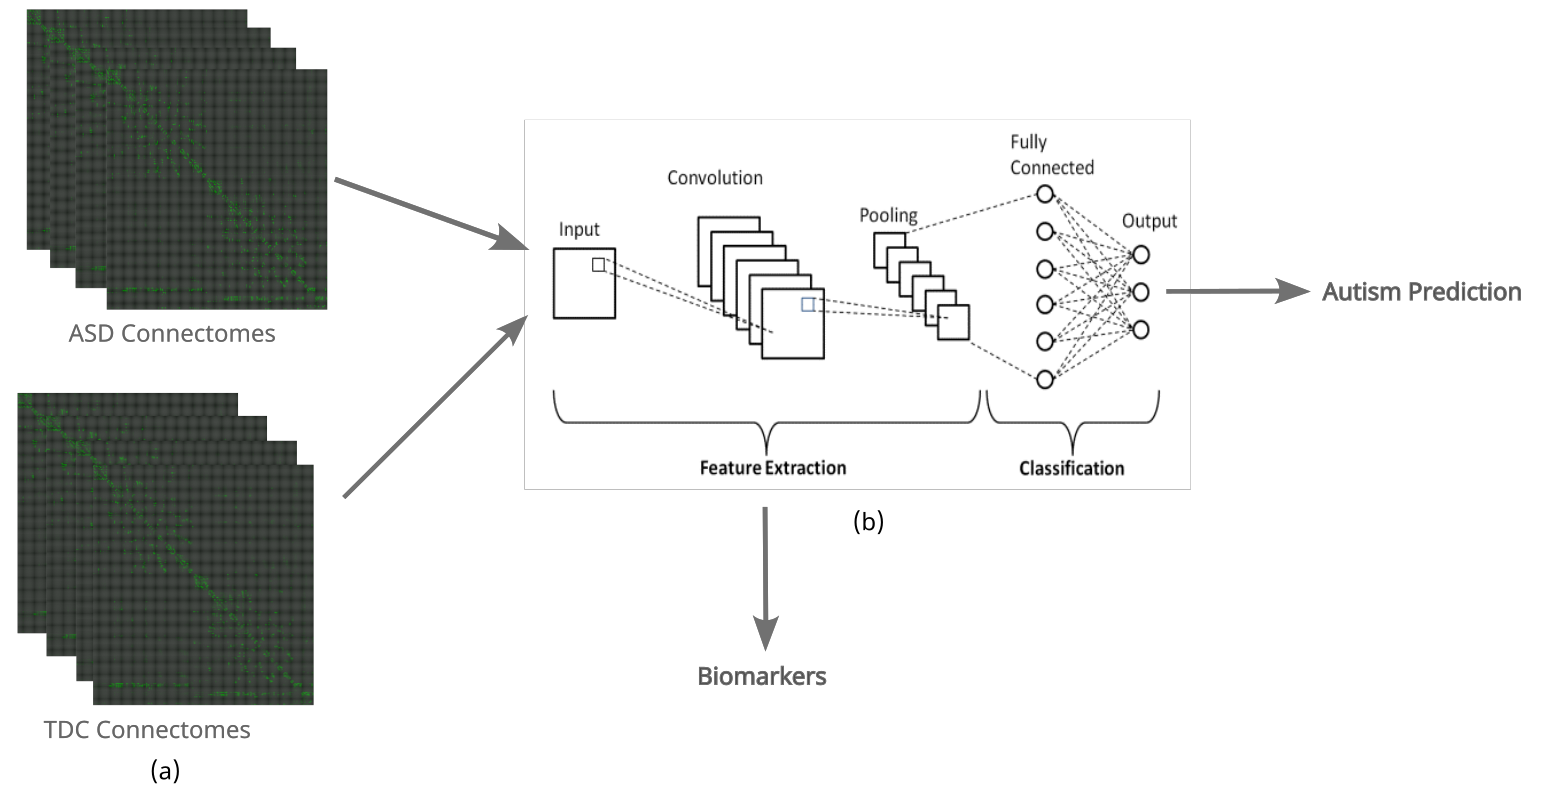
\includegraphics[width=\columnwidth]{../figures/project_schematic_v1.png}}
        \caption{Overview of autism prediction and biomarker identification using a Convolutional
                 Neural Network based classifier. (a) (top) Structural connectomes of patients 
                 with Autism Spectrum Disorder. (bottom) Structural connectomes of Typically 
                 Developing Controls. (b) Schematic diagram for convolutional neural network.}
        \label{project-schematic}
    \end{center}
    \vskip -0.2in
\end{figure}
